\chapter{مفاهيم اساسية}

\section{العلاقات والدوال}
\begin{definition}[( العلاقة ) \cite{elemrealanal}]
	اي مجموعة من الازواج المرتبة تسمى علاقة
\end{definition}
\noindent
\textbf{ملاحظة}\\
اذا كانت $S$ علاقة. فإن مجموعة كل العناصر التي تكن في المسقط الاول تسمى بالمجال. ومجموعة كل العناصر التي  تكون في المسقط الثاني تسمى بالمدى.

\begin{definition}[( الدالة ) \cite{elemrealanal}]
	الدالة $F$ هي مجموعة الازواج المرتبة $(x, y)$ بحيث لا يوجد زوجين مرتبين بنفس المسقط الاول. اي ان اذا كان
	$(x, y) \in F$ و $(x,z) \in F$
	فإن  $y=z$.
\end{definition}
\noindent
\textbf{ملاحظة}\\
تعريف الدالة يتطلب ان كل عنصر من المجال مثل $x$ يجب ان يوجد عنصر واحد فقط  مثل $y$ بحيث $(x,y)\in F$.\\
نسمي $y$ قيمة الدالة $F$ عند $x$ ونكتب
\[
y = F(x)
\] 

\begin{example}
	كل مما يأتي يمثل دالة على $\R$
	\begin{english}
			\begin{enumerate}[label=$\bullet$]
			\item $F=\{(x, y)\in \R\times\R : y = x^2\}$
			\item $G=\{(x, y)\in \R\times\R : y = \sin \sqrt{x^2-1}\}$
		\end{enumerate}
	\end{english}
ولكن المجموعات التالية لا تمثل دالة على $\R$
	\begin{english}
			\begin{enumerate}[label=$\bullet$]
		\item $A=\{(x, y)\in \R\times\R : x^2 + y^2 = 10\}$
		\item $B=\{(x, y)\in \R\times\R : x = \cos y\}$
	\end{enumerate}
\end{english}
لان 
$(1,3), (1,-3) \in A$
و
$(1, 0), (1, 2\pi) \in B$
\end{example}

\newpage
\section[الغاية و الاستمرارية]{الغاية و الاستمرارية \cite{mathanalysis}} 

\begin{definition}[( الغاية ) \cite{mathanalysis}]
	لتكن $f$ دالة معرفة على الفترة $(a, b)$. نفرض ان $c\in (a,b)$ اذا كان
	$f(x) \to A$ عندما $x\to c$ من خلال قيم اكبر من $c$ نقول ان $A$ هي غاية اليمين للدالة $f$ عند $c$ ونكتب
	\[
	\lim\limits_{x \to c^+} f(x) = A
	\]
	نرمز لغاية اليمين بالرمز $f(c^+)$ . بشكل ادق لكل $\epsilon>0$ يوجد $\delta>0$ بحيث
	\[
	|f(x) - f(c^+)| < \epsilon, \quad \text{if}\,\, c<x<c+\delta<b
	\]
\end{definition}
\noindent
\textbf{ملاحظة}\\
غاية اليسار تعرف بشكل مشابه اذا كانت $c\in (a, b)$ فإن غاية اليسار تعرف بالشكل 
\[
	f(c^-) = \lim\limits_{x \to c^-} f(x) = B
\]
حيث $x$ تاخذ قيم اصغر من $c$.
\begin{definition}[( الاستمرارية من اليمين)  \cite{mathanalysis}]
	اذا كانت الدالة $f$ معرفة عند $c$ وكان $f(c^+) = f(c)$ نقول ان $f$ مستمرة من اليمين عند $c$
\end{definition}

\begin{example}
	
الدالة $f(x) = \sqrt{x}$ تكون مستمرة من اليمين عند $x=0$ لأن
\[
f(0^+) = \lim\limits_{x \to 0^+} \sqrt{x} = 0 = f(0)
\]
\end{example}

\begin{definition}[( الاستمرارية من اليسار)  \cite{mathanalysis}]
اذا كانت الدالة $f$ معرفة عند $c$ وكان $f(c^-) = f(c)$ نقول ان $f$ مستمرة من اليسار عند $c$
\end{definition}
\noindent
\textbf{مثال}\\
الدالة $f(x) = \sqrt{-x}$ تكون مستمرة من اليسار عند $x=0$ لان
\[
f(0^-) = \lim\limits_{x \to 0^-} \sqrt{-x} = 0 = f(0)
\]
\newpage
\begin{definition}[( الاستمرارية ) \cite{mathanalysis}]
	اذا كانت $a<c<b$. فإننا نقول ان $f$ دالة مستمرة عند $x=c$ اذا وقثط اذا  كان
	\[
	f(c) = f(c^+) = f(c^-)
	\]
	اي تكون للدالة غاية من اليمين واليسار عند $c$ وكذلك تكون الدالة معرفة عند $c$.
\end{definition}

\begin{example}
الدالة $f(x) = \sqrt{x}$ غير مستمرة عند $x=0$ لان غاية اليسار غير موجودة وكذلك الدالة \\$ g(x) =- \sqrt{x}$ غير مستمرة عند $x=0$ لان غاية اليمين غير موجودة. ولكن الدالة المعرفة بالشكل
\[
F(x) = \begin{cases}
	\sqrt{x} & x\geq0 \\
	-\sqrt{x} & x < 0
\end{cases}
\]
تكون مستمرة عند $x=0$ لان
\[
f(0^+) = f(0^-) = 0 = f(0)
\]

\begin{figure}[H]
	\centering
		\begin{tikzpicture}
		\begin{axis}[
			axis lines = middle,
			xlabel = \( x \),
			ylabel = \( F(x) \),
			domain = -5:5,
			samples = 100,
			]
			\addplot[blue, thick,domain=0:5] {sqrt(x)};
			\addplot[red, thick,domain=-5:0] {sqrt(-x)};
		\end{axis}
	\end{tikzpicture}
\end{figure}
\end{example}
\newpage
\section[المشتقة]{المشتقة \cite{realanal}}
\begin{definition}
	لتكن $f$ دالة معرفة على الفترة المفتوحة $(a, b)$ ولتكن $c\in (a, b)$ فإن $f$ تكون قابلة للاشتقاق عند $c$ اذا كانت الغاية
	\[
	f'(c) = \lim\limits_{x\to c} \frac{f(x) - f(c)}{x-c} 
	\]
	موجودة. وتسمى المشتقة للدالة $f$ عند $c$.
\end{definition}


\section[التقارب للدوال]{التقارب للدوال \cite{elemrealanal}} 
لتكن $A\subseteq\R$ ونفرض ان لكل $n\in\N$ توجد دالة $f_n:A\to\R$ سوف نقول ان $(f_n)$ متتابعة من الدوال على $A$.
\begin{definition}[{[التقارب النقطي] \cite{elemrealanal}}]
 	لتكن $(f_n)$ متتابعة من الدوال على $A\subseteq\R$. لتكن $A_0\subseteq A$ ولتكن $f:A_0\to\R$. نقول ان المتتابعة $(f_n)$ تتقارب نقطياً الى الدالة $f$ اذا كان لكل $x\in A_0 $ فإن المتتابعة $f_n(x)$ تتقارب الى $f(x)$.
\end{definition}

\begin{example}
	 لتكن لدينا المتتابعة من الدوال
	\[
	f_n(x) = \frac{x}{n}
	\]
	ولتكن $f(x) = 0$ لكل $x\in \R$. نلاحظ ان لكل $x\in \R$
	\[
	\lim\limits_{n\to \infty}f_n(x)  = \lim\limits_{n\to \infty}\frac{x}{n} = 0 = f(x)
	\]
	\end{example}
\begin{example}
لتكن لدينا المتتابعة 
	\[
	g_n(x) = \frac{x^2 + nx}{n}
	\]
	ولتكن $g(x) = x$. فإن لكل $x\in\R$
	\[
	\lim\limits_{n\to \infty}g_n(x)  = \lim\limits_{n\to \infty}\frac{x^2+nx}{n} = \lim\limits_{n\to \infty}\frac{x^2}{n} + x = x = g(x)
	\]
\end{example}

\begin{definition}[{[التقارب المنتظم]} \cite{elemrealanal}]
	متتابعة من الدوال $(f_n)$ على $A\subseteq\R$ تقترب بشكل منتظم الى الدالة $f:A_0\to\R$ اذا كان لكل $\epsilon>0$ يوجد عدد طبيعي $K(\epsilon)$ بحيث اذا كان $n\geq K(\epsilon)$ فإن 
	\[
	|f_n(x) - f(x) | < \epsilon, \quad \text{لكل $x\in A_0$}
	\]
\end{definition}

\begin{note}
	التقارب المنتظم يحافظ على استمرارية الدالة. اي اذا كانت لدينا متتابعة من الدوال المستمرة فإن التقارب المنتظم لها هو دالة مستمرة.
\end{note}

\section[التكامل]{التكامل \cite{introrealanal}}

سوف نتعامل مع الدوال المعرفة على الفترة المغلقة $[a, b]$ ، التجزئة للفترة عبارة عن فترات 
\begin{equation}
	[x_0, x_1],\, [x_1, x_2],\, \dots, [x_{n-1}, x_n]
\end{equation}
حيث
\begin{equation}
	a = x_0 < x_1 < x_2 < \cdots < x_n=b
\end{equation}
نرمز للتجزئة بالرمز 
\[
P = \{x_0 , x_1, \dots, x_n\}
\]
اكبر طول من اطوال الفترات الجزئية في (1) يكون طول التجزئة، ويكتب بالشكل
\[
||P|| = \max_{1\leq i \leq n} (x_i - x_{i-1})
\]
اذا كانت $f$ معرفة على الفترة $[a, b]$ ، فإن المجموع
\[
\sigma = \sum_{j=1}^{n} f(c_j) (x_j - x_{j-1})
\]
حيث
\[
x_{j-1} \leq c_j \leq x_j , \quad 1\leq j \leq n
\]
يسمى مجموع ريمان للدالة $f$ على التجزئة $P$

\begin{definition}[( تكامل ريمان ) \cite{introrealanal}]
	لتكن $f$ دالة معرفة على الفترة $[a, b]$ ، نقول ان $f$ دالة قابلة لتكامل ريمان على الفترة $[a, b]$ اذا وجد عدد $L$ يحقق الآتي: لكل $\epsilon> 0 $ يوجد $\delta < 0 $ بحيث
	\[
	|\sigma - L |< \epsilon
	\]
	حيث $\sigma$ هو اي مجموع ريمان على التجزئة $P$ للفترة $[a, b]$ بحيث ان $||P|| > \delta$ في هذه الحالة نقول $L$ هو تكامل ريمان للدالة $f(x)$ على الفترة $[a, b]$ ونكتب
	\[
	\int_{a}^{b} f(x)\, dx = L
	\]
\end{definition}

\begin{definition}[( التكامل العلوي والسفلي ) \cite{introrealanal}]
	اذا كانت $f$ دالة مقيدة على الفترة $[a, b]$ و $P = \{x_0, x_1, \dots, x_n\}$ هي تجزئة للفترة ، لتكن 
	\[
	M_j = \sup_{x_{j-1}\leq x\leq x_j} f(x)
	\]
	و
	\[
	m_j = \inf_{x_{j-1}\leq x\leq x_j} f(x)
	\]
	المجموع العلوي للدالة $f$ على $P$ يكون
	\[
	S(P) = \sum_{j=1}^{n} M_j (x_j - x_{j-1})
	\]
	و التكامل العلوي يكون القيمة الصغرى لجميع المجاميع العلوية ويرمز له بالرمز
	\[
	\overline{
	\int_{a}^{b} 
	}
	f(x)\, dx
	\]
	المجموع السفلي للدالة $f$ على $P$ يكون
	\[
	s(P) = \sum_{j=1}^{n} m_j (x_j - x_{j-1})
	\]
	و التكامل السفلي يكون القيمة العظمى لجميع المجاميع السفلية ويرمز له بالرمز
	\[
	\underline{
		\int_{a}^{b} 
	}
	f(x)\, dx
	\]
\end{definition}

\begin{figure}[H]
	\centering
	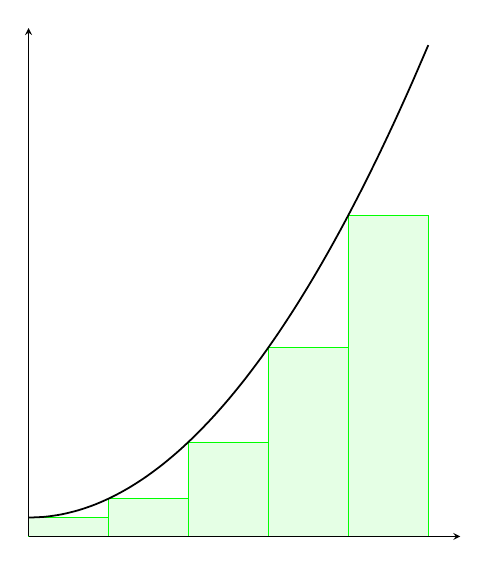
\begin{tikzpicture}[scale=0.8]
\begin{axis}[
xtick=\empty, ytick=\empty,
	y=0.3cm, xmax=5.4,ymax=26.9,ymin=0,xmin=0,
	enlargelimits=true,
	axis lines=middle,
	clip=false,
	domain=0:5,
	axis on top
	]
	\addplot [draw=green, fill=green!10, ybar interval, samples=6]
	{1+x^2}\closedcycle;
	\addplot[smooth, thick,domain=0:5]{1+x^2};
\end{axis}
\end{tikzpicture}
\caption{المجموع السفلي}
\end{figure}

\begin{figure}[H]
	\centering
	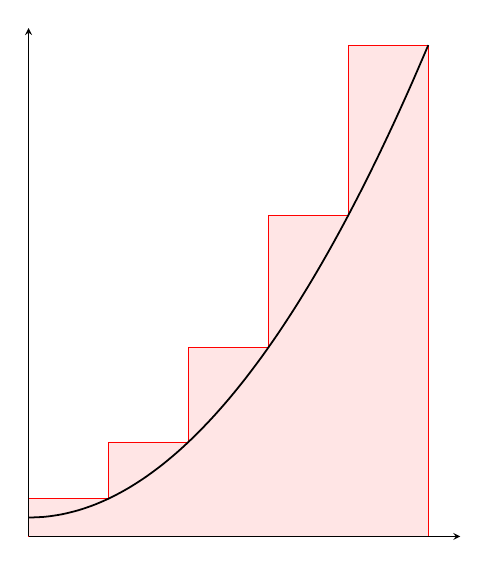
\begin{tikzpicture}[scale=0.8]
	\begin{axis}[
xtick=\empty, ytick=\empty,
		y=0.3cm, xmax=5.4,ymax=26.9,ymin=0,xmin=0,
		enlargelimits=true,
		axis lines=middle,
		clip=false,
		domain=0:5,
		axis on top
		]
		\addplot [draw=red,fill=red!10,const plot mark right, samples=6]
		{1+x^2}\closedcycle;
		\addplot[smooth, thick,domain=0:5]{1+x^2};
	\end{axis}
\end{tikzpicture}
\caption{المجموع العلوي}
\end{figure}